\chapter*{Konzeptentwurf}
\label{cha:Konzeptentwurf}

\section*{State Machine}
\label{sec:State Machine}

\subsection*{Initialzustand}
\label{subsec:Initialzustand}

Das System startet im Initialzustand und wechselt direkt in den sogenannten Idle-Zustand. Im Idle-Zustand sind beide LEDs der Anzeige AC2398 ausgeschaltet. In diesem Zustand kann das System je nach den erkannten Eingaben oder Ereignissen in andere Zustände wechseln. Wenn der grüne Knopf gedrückt wird und kein RFID-Tag erkannt wird, speichert das System die aktuelle Systemzeit und bleibt im Idle-Zustand. Dieser Vorgang wird im Diagramm als "Save Time" bezeichnet.

\subsection*{Tag-Erkennung und Verarbeitung}
\label{subsec:Tag-ErkennungundVerarbeitung}

Wird ein NFC-Tag erkannt und liegt kein Fehlerzustand vor, wechselt das System in den Zustand "Tag Detected Handling". In diesem Zustand blinkt die grüne LED mit einer Frequenz von einer Sekunde, um anzuzeigen, dass ein Tag erkannt wurde. Es gibt zwei mögliche Aktionen, vorausgesetzt, es liegt kein Fehlerzustand vor:

Write Tag Handling: Wenn der grüne Knopf gedrückt wird, während das RFID-Tag erkannt wird und die Systemzeit vorhanden ist, wechselt das System in den Zustand "Write Tag Handling". In diesem Zustand wird die zuvor gespeicherte Systemzeit auf das RFID-Tag geschrieben. Die grüne LED leuchtet dauerhaft, um anzuzeigen, dass der Schreibvorgang erfolgreich abgeschlossen wurde. Sobald das RFID-Tag nicht mehr erkannt wird, kehrt das System in den Idle-Zustand zurück.

Delete Tag Handling: Alternativ kann der rote Knopf gedrückt werden, während das RFID-Tag erkannt wird und kein Fehlerzustand vorliegt. In diesem Fall wechselt das System in den Zustand "Delete Tag Handling". Hier werden die gespeicherten Daten des RFID-Tags gelöscht, und beide LEDs leuchten dauerhaft, solange das Tag erkannt wird. Sobald das RFID-Tag nicht mehr erkannt wird, kehrt das System in den Idle-Zustand zurück.

\subsection*{Fehlerbehandlung}
\label{subsec:Fehlerbehandlung}

Wenn während des Prozesses ein Fehlerzustand auftritt, wechselt das System in den Zustand "Error State Handling". In diesem Zustand blinkt die rote LED mit einer Frequenz von einer Sekunde, während die grüne LED ausgeschaltet bleibt, um den Fehler anzuzeigen. Der Fehlerzustand bleibt bestehen, bis die Ursache des Fehlers behoben ist. Anschließend erreicht das System den Finalzustand und der gesamte Ablauf beginnt erneut.
\begin{figure}[h!]
	\centering
	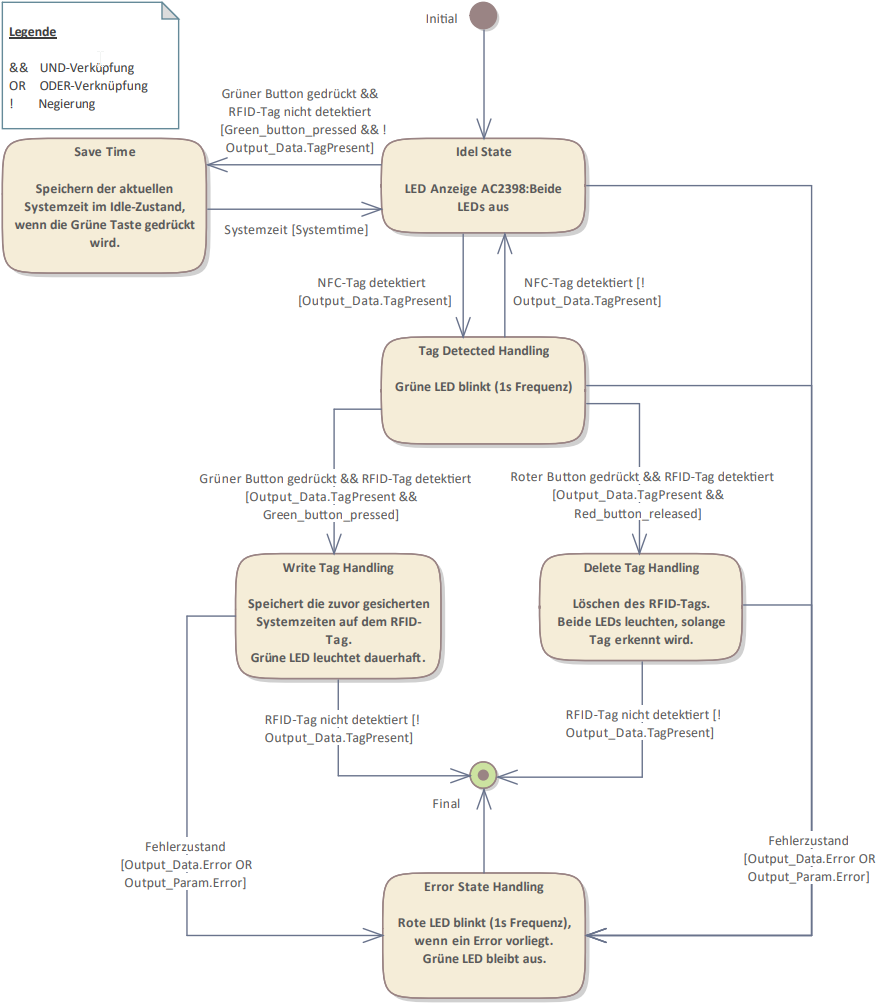
\includegraphics[width=1.0\textwidth]{images/StateMachine.png}
	\vspace{1cm}
	\caption{State-Machine-Diagramm}
	% [Abbildungsverzeichnis]{Bildunterschrift}
	\label{fig:StateMachineDiagramm}
\end{figure}

\clearpage
\begin{comment} % Aus Angabe:
Erstellung eines Konzept (Planung) mit geeigneter (kompakter) Dokumentation \newline
* Signalliste \\
* Statemachine \\
\end{comment}
\begin{table}[h!]
	\centering
	\renewcommand{\arraystretch}{1.0} % Verringert den Zeilenabstand
	\footnotesize
	\begin{tabular}{|l|l|l|l|}
		\hline
		\textbf{Name} & \textbf{Datentyp} & \textbf{Adresse} & \textbf{Kommentar}\\ \hline
		RED\_button\_released & Bool & \%I193.2 & 1 wenn roter Taster nicht gedrückt \\ \hline
		Green\_button\_pressed & Bool & \%I193.3 & 1 wenn grüner Taster gedrückt \\ \hline
		Red\_button\_LED\_ON & Bool & \%Q192.0 & wenn 1 dann rote LED vom Taster an \\ \hline
		Green\_button\_LED\_ON & Bool & \%Q192.1 & wenn 1 grüne LED vom Taster an \\ \hline
	\end{tabular}
	\caption{Variablentabelle von AC2398 (Tasterblock)}
	\label{tab:AC2398}
\end{table}
\begin{table}[h!]
	\centering
	\renewcommand{\arraystretch}{1.0} % Verringert den Zeilenabstand
	\footnotesize
	\begin{tabular}{|l|l|l|l|}
		\hline
		\textbf{Name} & \textbf{Datentyp} & \textbf{Adresse} & \textbf{Kommentar} \\ \hline
		Output\_Param.Done & Bool & \%I6.0 & \\ \hline
		Output\_Param.Busy & Bool & \%I6.1 & \\ \hline
		Output\_Param.Error & Bool & \%I6.2 & \\ \hline
		Output\_Param.Status & Word & \%IW8 & \\ \hline
		Output\_Param.ExtStatus & DWord & \%ID10 & \\ \hline
		Output\_Param.RdValue & UInt & \%IW14 & \\ \hline
		Output\_Data.TagPresent & Bool & \%I92.0 & \\ \hline
		Output\_Data.Done & Bool & \%I92.1 & \\ \hline
		Output\_Data.Busy & Bool & \%I92.2 & \\ \hline
		Output\_Data.Error & Bool & \%I92.3 & \\ \hline
		Output\_Data.Status & Word & \%IW94 & \\ \hline
		Output\_Data.ExStatus & Word & \%IW96 & \\ \hline
		Input\_Param.Execute & Bool & \%Q0.0 & \\ \hline
		Input\_Param.Mode & UInt & \%QW2 & \\ \hline
		Input\_Param.SetValue & UInt & \%QW4 & \\ \hline
		Input\_Data.DT\_InAddr & UInt & \%QW16 & \\ \hline
		Input\_Data.DT\_OutAddr & UInt & \%QW18 & \\ \hline
		Input\_Data.Execute & Bool & \%Q20.0 & \\ \hline
		Input\_Data.Force & Bool & \%Q20.1 & \\ \hline
		Input\_Data.Mode & UInt & \%QW22 & \\ \hline
		Input\_Data.TagMemAddr & UInt & \%QW24 & \\ \hline
		Input\_Data.Length & UInt & \%QW26 & \\ \hline
		Input\_Data.WrData & Array[0..31] of Byte & \%Q28.0 & \\ \hline
		Input\_Data.RdData & Array[0..31] of Byte & \%Q60.0 & \\ \hline
	\end{tabular}
	\caption{Variablentabelle von DTI515 (NFC-Modul)}
	\label{tab:DTI515}
\end{table}

\clearpage

% ------------------------------------------------------------------------------------
%... Text Konzeptentwurf: Gegenüberstellung verschiedener Lösungsansätze und Lösungsgenerierung, etc.